\begin{figure}[h]
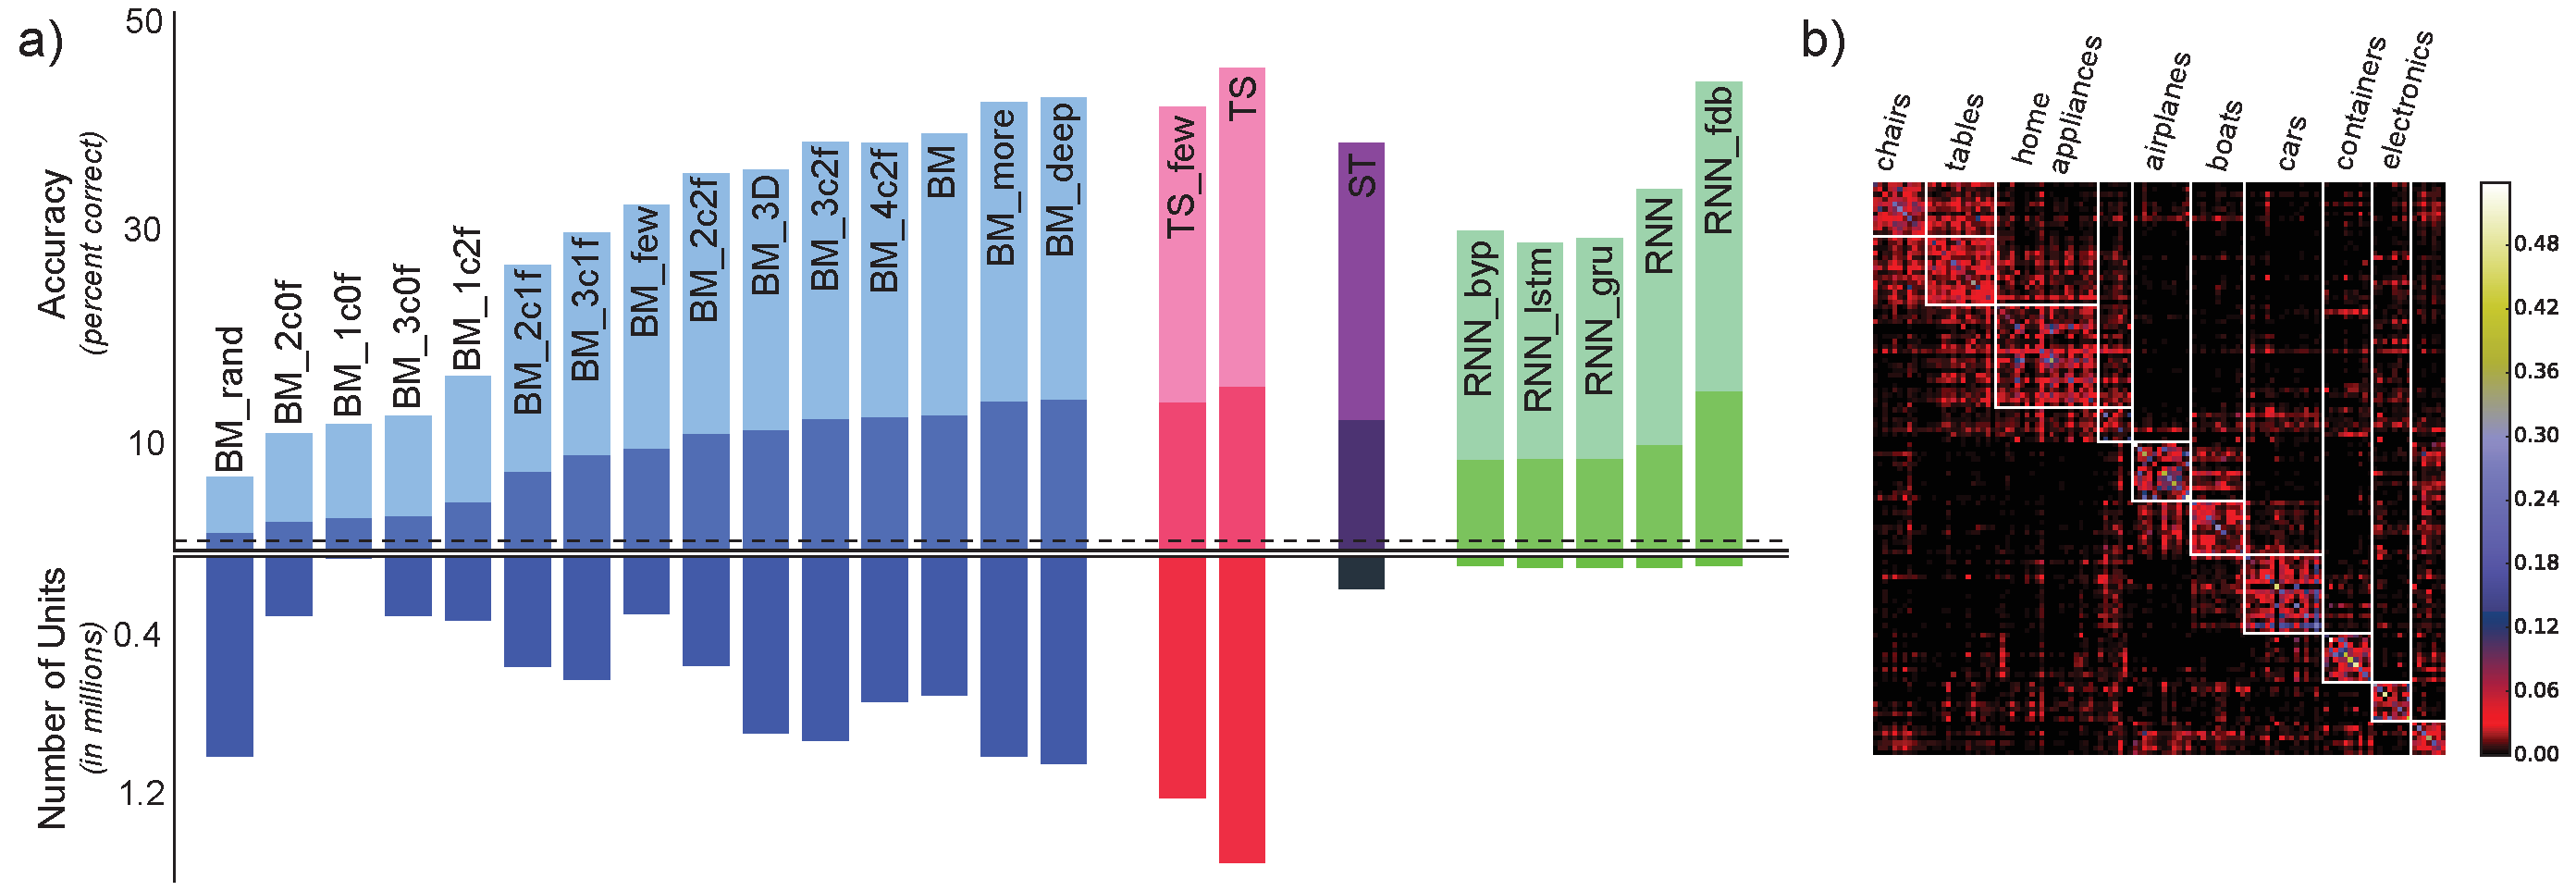
\includegraphics [width=1\linewidth]{figures/results.pdf}
\vspace{-2mm}
\caption{\textbf{Performance results.} \textbf{a.} Each bar in this figure represents one model. The positive $y$-axis is performance measured in percent correct (top1=dark bar, chance=0.85\%, top5=light bar, chance=4.2\%).   The negative $y$-axis indicates the number of units in networks, in millions of units. Model architecture family is indicated by color.  The definition of individual model labels can be found in the Results section. \textbf{b.} Confusion Matrix.~\label{fig_main}}
\end{figure}

Our strategy in identifying potential models of barrel cortex is to explore each family in terms of its ability to solve the shape recognition task in our training set, evaluating both performance and efficiency (e.g. number of units needed). 
Realizing that comparing models with different number sof parameters may be unfair, we generally controlled all models evaluated to have roughly numbers of parameters, with exceptions where noted.  
We evaluated many individual structures within each family (Fig. \ref{fig_main}). 
Our results can be summarized with following conclusions:

\begin{itemize}
   \item Most network choices within all families do a poor job at the task, achieving chance or just-above-chance performance. 
   However, within each family, certain specific choices of parameters lead to much better network performance.
   \item Overall, the best performance was obtained for an instance of the Temporal-Spatial model, with 15.2\% top-1 and 44.8\% top-5 accuracy.  
   Visualizing a confusion matrix (Fig. \ref{fig_main})b indicates that errors are largely reasonable. 
   \item In general, increasing the depth of the architecture was helpful, with architectures with fewer than four convolutional layers achieving much lower performance than somewhat deeper ones.
   \item In general, increasing the number of parameters were somewhat helpful, but only to a point. 
   The Temporal-Spatial architecture, was able to outperform other classes while using significantly fewer parameters. 
   \item Recurrent networks with long-range feedback were able to perform nearly as well as the Temporal-Spatial model with equivalent numbers of parameters, while using far fewer units.   
   These long-range feedbacks appeared critical to performance, with purely local recurrent architectures (including LSTM and GRU) achieving significantly worse results.
\end{itemize}
 

\subsection{Specific Models}

[List of specific model names and architectures.]
